% !TEX encoding = UTF-8 Unicode
\documentclass{sig-alternate}
\usepackage{textcomp}
\usepackage{graphics}
\usepackage[utf8]{inputenc}
\usepackage[T1]{fontenc}

\hyphenation{li-neal co-rrec-ci\'on pro-ble-ma Back-propagation con-si-de-ra}

\begin{document}

\pagenumbering{arabic}

\title{Aprendizaje Supervisado en Redes Neuronales Multicapa}
\subtitle{Sistemas de Inteligencia Artifical - ITBA}

\numberofauthors{3}

\author{
	\alignauthor{Carlos Sessa}\\
	\alignauthor{Lucas Pizzagalli}\\
	\alignauthor{Nicolás Purita}\\	
}

\date{3 de Mayo de 2012}

\maketitle

\section*{Introducción}

	Se implementó una red neuronal multicapa supervisada para resolver una función con la siguiente forma:

	\begin{figure}[!ht]
		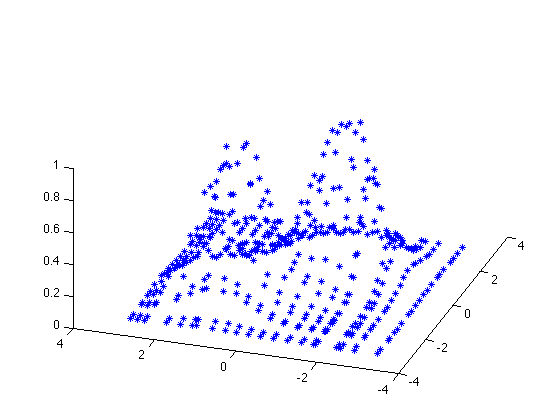
\includegraphics[scale=0.5]{./figures/function.png}
  		\caption{Distribución de puntos dada}
  		\label{fig:function}
	\end{figure}

	En la figura \ref{fig:function} se puede observar que los puntos de la entrada pertenecen al intervalo $[-3.5, 3.5]$ y la salida se encuentra en el intervalo $(0, 1)$.\\
	La implementación de la red fue realizada en \textit{Matlab}. Se corren distintos experimentos, variando las parámetros y arquitecturas a fin de optimizar la generalización del problema. También se implementan dos mejoras al algoritmo para verificar aumentar la capacidad de la red de generalizar en menor tiempo y en forma óptima.

\section*{Desarrollo y Problemas encontrados}

	Los pesos se ajustan utilizando el algoritmo de \textit{Backpropagation} y los patrones son presentados a la red en orden aleatorio durante el aprendizaje. Como condición de parada se considera una cota superior para el error ($0.01$) y a la vez una cota para el número de épocas ($350$) para el entrenamiento. Se realizaron varias corridas modificando los parámetros para analizar correctamente el problema. Teniendo en cuenta como los parámetros afectan la eficacia y performance de la red, eligiendo finalmente el que proporciona la mejor solución.\\

	Un tema a destacar es la división y selección de los puntos de entradas, estos son divididos en \textit{Puntos de entrenamiento} y \textit{Puntos de Testeo}. Los puntos de entradas son cargados desde un archivo en donde se encuentran exactamente $441$ puntos de la función, distribuidos uniformemente sobre el dominio. El criterio con el que se seleccionan los patrones es el siguiente, el $80\%$ es tomado para el grupo de \textit{Patrones de entrenamiento} y el $20\%$ restante corresponden al \textit{Puntos de Testeo}. Dado que los puntos dentro del archivo se encontraban distribuidos en forma aleatoria se crean los dos subconjuntos utilizando un random.

	\begin{figure}[!ht]
		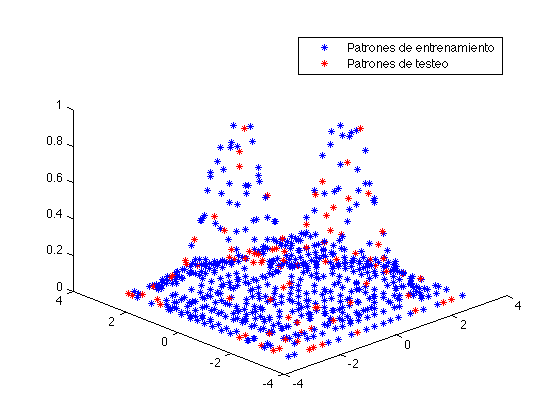
\includegraphics[scale=0.5]{./figures/muestreo.png}
	  	\caption{Distribución de puntos de entrenamiento y puntos de testeo.}
	  	\label{fig:input}
	\end{figure}
	
	En la figura \ref{fig:input} se puede ver los dos subconjuntos, el de \textit{entrenamiento} y \textit{testeo}. De esta forma verificamos las distribución de los puntos y podemos deducir que el conjunto de \textit{testeo} es bueno\footnote{Un conjunto de puntos es \textbf{bueno} si cubre la mayor superficie de la función.}.\\
	Durante el desarrollo y en la búsqueda de la mejor arquitectura surgió el problema de que habían muchos puntos sobre la superficie de la función por lo que decidimos tomar todos los puntos de la superficie que cumplan la condición de $z \geq 0.01$. De esta forma no tenemos tanta densidad de puntos sobre la superficie. En la figura \ref{fig:input2} se puede observar la nueva distribución de puntos para entrenar la red.

	\begin{figure}[!ht]
		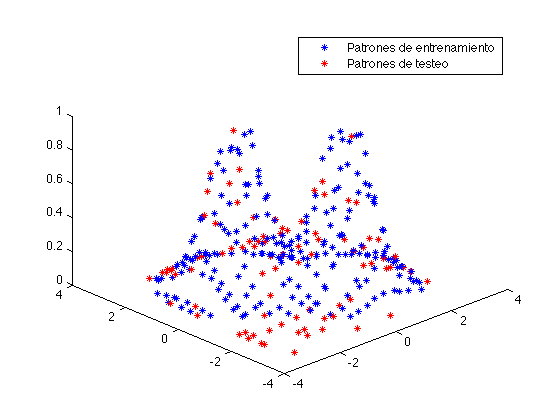
\includegraphics[scale=0.5]{./figures/muestreo2.png}
		\caption{Distribución de puntos tomando los mayores a $0.01$}
		\label{fig:input2}
	\end{figure}

	Un tema a destacar es la utilización de la función de activación $g(x) = tanh(\beta x)$ en la última capa. Sucede que el intervalo de salida de la función dada pertenece al $(0,1)$ por ende se dedujo que sería más apropiado poner una función \textit{exponencial} o \textit{lineal} en la última capa, a comparación de la función \textit{tangencial} que tiene su imagen en el intervalo $(-1,1)$. \\

	Los pesos iniciales se generan de forma aleatoria en el intervalo $[-0.5,0.5]$. Por último, es necesario mencionar que el orden en que se le dan los patrones a la red durante el entrenamiento es aleatorio.
	
\section*{Resultados y Conclusiones}

	Para el $\eta-adaptativo$ se realizaron muchas variantes de los parámetros para ir ajustando los valores. Estos valores no son presentados en el informe ya que se deciden en función de la performance y comportamiento de la red. La variable de incremento del $\eta$ es fija, esto quiere decir que se incrementa en $0.01$ cada vez que sea necesario y se decrementa en un $5\%$ del valor del $\eta$ actual. Para el \textit{Momentum}, luego de probar distintos valores, se tomó el mejor valor como $\alpha = 0.1$. \\
	Para comparar la red entre distintas arquitecturas, se le enseña a la red con los mismos pesos iniciales y en un lapso de tiempo de $350$ épocas. Se consideran en todas las arquitecturas $2$ neuronas de entradas y $1$ de salida.\\

	\begin{table}[h]
		\begin{center}
			\begin{tabular}{ | p{2cm} | p{1.5cm} | }
				\hline
				Arquitectura & Error \\ \hline
				$[30\,20\,10]$ & 0.0290183  \\ 
				\hline
				$[10\,10]$ & 0.0462676  \\ 
				\hline
				$[10]$ & 1.65359  \\ 
				\hline
				$[10\,10\,10\,10]$ & 0.05552  \\ 
				\hline
				$[40\,20]$ & 0.115901  \\ 
				\hline
				$[10\,10\,10]$ & 0.081405  \\ 
				\hline
				$[5\,10\,20]$ & 0.405984  \\ 
				\hline	
			\end{tabular}
			\caption{Tabla de comparaciones entre distintas arquitecturas}	
			\label{t:arquis}
		\end{center}
	\end{table}

	Las arquitecturas mostradas en la tabla \ref{t:arquis} poseen en las capas ocultas la función de activación \textit{exponencial} y en la última capa tiene configurado para utilizar una función de activación \textit{lineal}. La función de activación \textit{exponencial} es configurada con un $\beta = 2$, este valor se obtuvo mediante pruebas y verificando la performance de la red. \\

	La configuración de la fila 1 de la tabla \ref{t:arquis}, se observa que es la red con menor error de entrenamiento obtenido. Con el objetivo de visualizar mejor que representa dicho error, se ha generado la figura \ref{fig:errorEsperadoReal}. En dicha figura se puede apreciar que la red ha aprendido bastante ya que la relación entre valor esperado y valor obtenido por la red se asemejan mucho en la mayoría de los casos. Los puntos generan una figura que es muy similar a una recta (la recta es el caso ideal, en el que los datos obtenidos son iguales a los reales). De todos modos se aprecia que al cabo de $350$ épocas existen algunos patrones que aún no fueron aprendidos, en particular los patrones de los picos de la función. Una forma de mejorar el aprendizaje es modificando los puntos de tal forma de que haya mas concentración de puntos de entrenamiento en los picos. Luego de $350$ épocas se obtiene un error de entrenamiento de $0.0290183$.\\


	En la figura \ref{fig:errorsByEpochs} se puede ver como evolucionan los errores a medida que transcurre el tiempo. A simple vista se observa como al principio el error de los patrones de testeo es menor a los patrones de entrenamiento. Esto se debe a que todavía la red no ajustó los pesos lo suficiente pero a medida que la misma aprende lo suficiente se ve como el error de entrenamiento desciende por debajo del error de testeo.\\

	\begin{table}
		\begin{center}
			\begin{tabular}{ |p{0.5cm}|p{2cm}|p{2cm}|p{2cm}| }
				\hline
				$\eta$ & \textit{Momentum} & Error entrenamiento & Error testeo \\ \hline
				No & No & 0.0304268 & 0.0949303 \\ 
				\hline
				Sí & No & 0.0441066 & 0.0902171 \\
				\hline
				No & Sí & 0.0325069 & 0.0839944 \\
				\hline
				Sí & Sí &  0.0290183 & 0.0762365\\
				\hline
			\end{tabular}
			\caption{Mejor configuración con y sin mejoras}
			\label{t:bestConf}
		\end{center}
	\end{table}
	
	En la Tabla \ref{t:bestConf} se puede observar como el $\eta-adaptativo$ y el \textit{Momentum} mejoran la performance y el conocimiento de la red.

	\begin{figure}[!ht]
		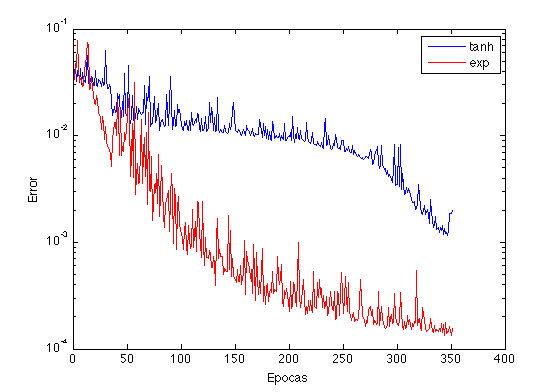
\includegraphics[scale=0.5]{./figures/tanVsExp.png}
	  	\caption{Comparación entre la tangencial y exponencial}
	  	\label{fig:tanVsExp}
	\end{figure}

	En la figura \ref{fig:tanVsExp} se puede ver como, utilizando la \textit{exponencial} como función de activación, en las capas ocultas se logra un mejor resultado que utilizando la \textit{tangencial}.

\newpage
\onecolumn

\begin{figure}[!ht]
	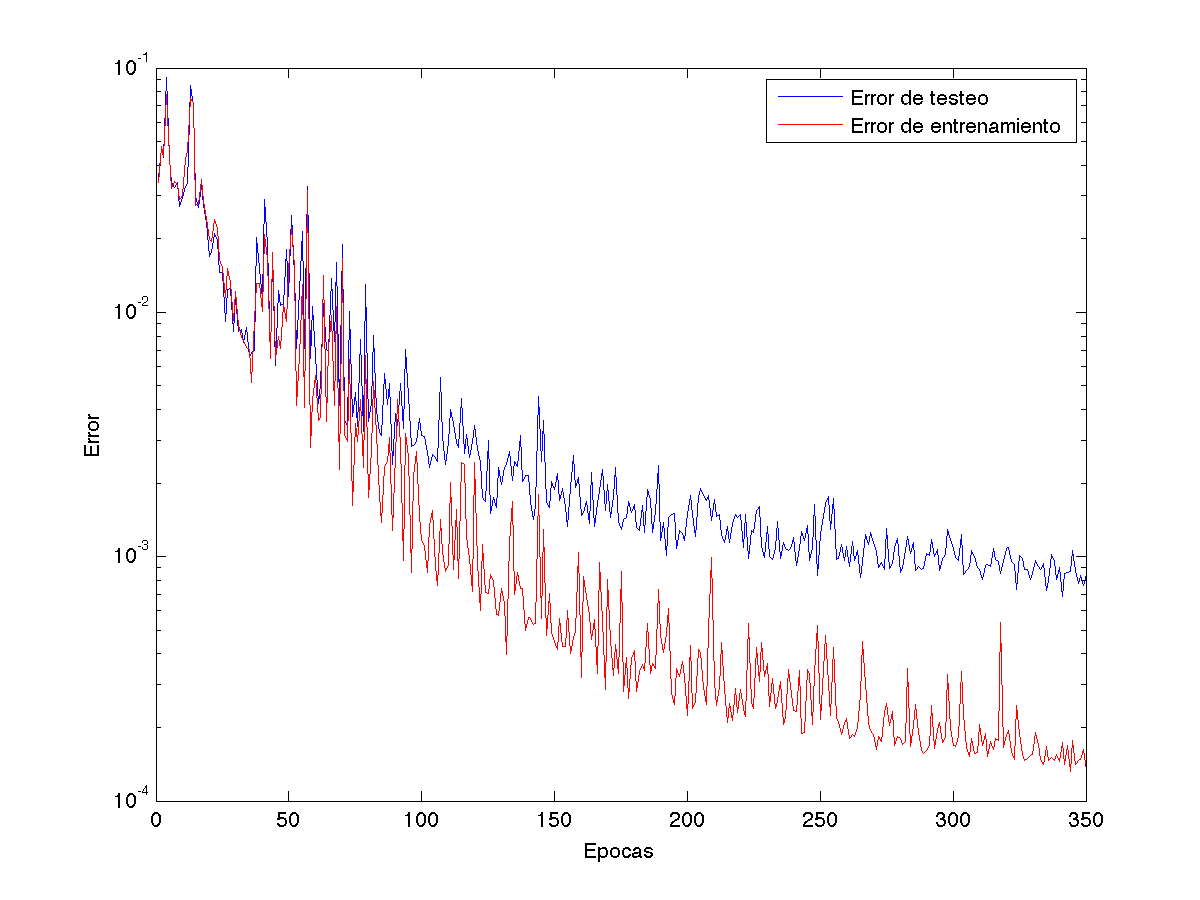
\includegraphics[scale=0.8]{./figures/mejorErrores.png}
  \caption{Evolución de error de testeo y entrenamiento durante el entrenamiento}
  \label{fig:errorsByEpochs}
\end{figure}


\begin{figure}[!ht]
	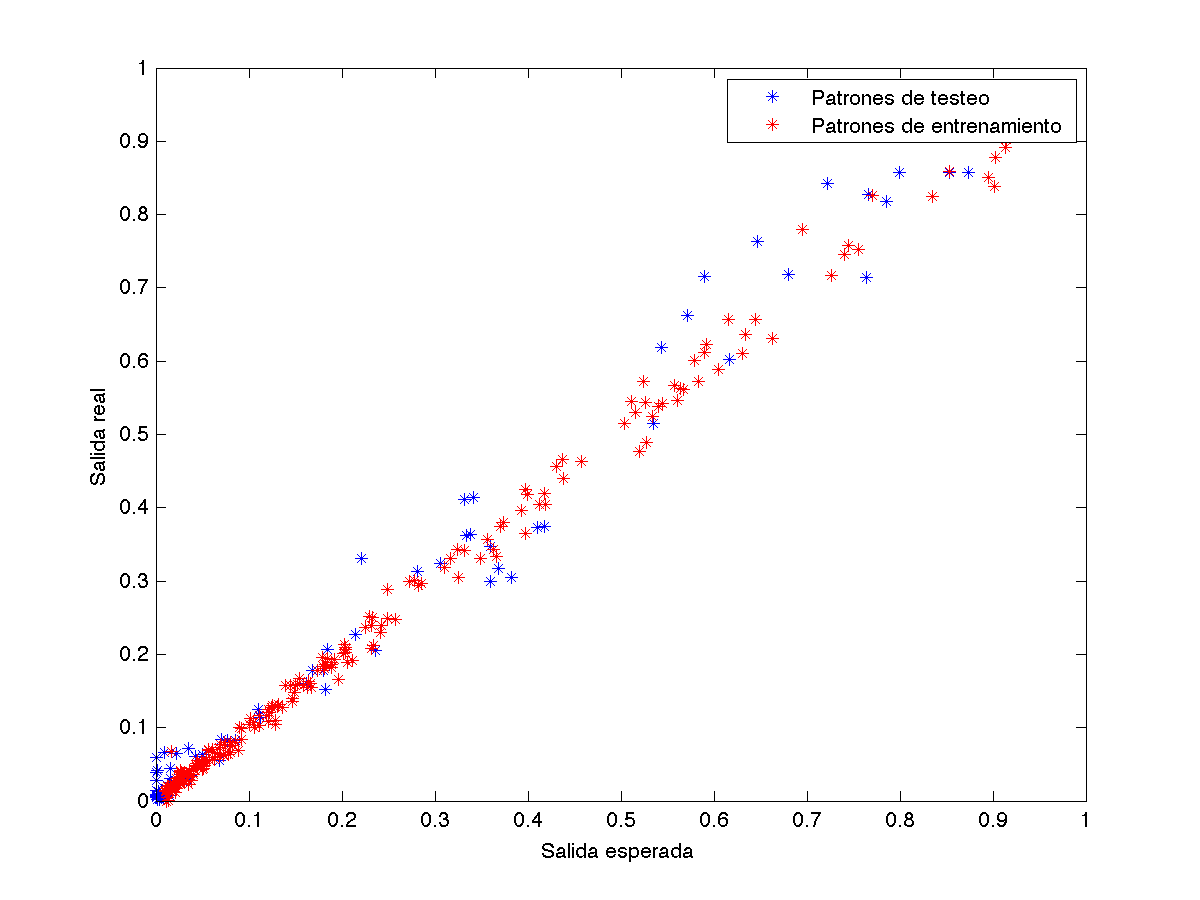
\includegraphics[scale=0.8]{./figures/mejorRealVsEsperada.png}
  \caption{Comparación entre salidas esperadas y obtenidas}
  \label{fig:errorEsperadoReal}
\end{figure}

\end{document}
